\section{Theory}
\paragraph{Gamma decay}
Radioactive decay is the process by which an unstable atom[nucleus?] transitions to a more stable form through the emission of energy by radiation.
Decay occurs in three main forms[kinds], each associated with a radiation of different nature and properties: $\alpha$-decay, $\beta$-decay and $\gamma$-decay.

$\alpha$-decay represents the disintegration of a parent nucleus to a daughter through the emission of a nucleus of a helium atom (an $\alpha$ particle).
$\beta$-decay is the transformation of a nucleus with an unstable ratio of protons to neutrons into a stabler one by emitting an electron ($\beta^-$ particle), in the case of a proton-rich nucleus, or a positron ($\beta^+$ particle), in the case of an over-abundance of neutrons.
Additionally, a proton-rich nucleus can also reduce its charge by the absorption of an atomic electron, in a process called \emph{electron capture}.
The electron comes most often from the inner $K$-shell, resulting in the outer electrons cascading down to fill the lower levels and emitting [one or more] X-rays\cite{intro_nuclear_particle_physics}.

\paragraph{Scintillation detector}
Scintillation detectors are based on the properties of scintillators, materials that emit photons in the visible spectrum after the passage of a charged particle.
The scintillators used for particle detection are primarily [split] between two types: organic (or plastic), in which the photon emission has molecular origin, 
and inorganic (or crystalline), crystals which are doped with activators that can first be excited by electron-hole pairs 
produced by the charged particle passing in the crystal lattice\footnotemark\ and then de-excited by photon emission\cite{intro_nuclear_particle_physics}.

Because of the low intensity of the emitted light, the photon signal must be amplified in order to be properly counted.
This amplification is commonly achieved through the use of photomultiplier tubes (PMT), a device which converts the photon signal in a detectable electric pulse.
It consists of a vacuum chamber containing several components, pictured in Fig. \ref{fig:photomultiplier}: 
after passing a transparent entry window, adjacent to the scintillator, the scintillation photons first encounter a photocatode, 
where they produce an electron by photoelectric effect with a certain probability $\varepsilon$ (the quantum efficacy).
Next, a series of dynodes accellerate the electrons and multiply them through secondary emission.
The anode located at the end of the chamber then allows to read the amplified electric signal, 
which results linearly proportional to the amount of light incident on the photocathode.
The voltage applied between cathode and anode determines the value of the total gain $G$.
\footnotetext{Ici je pourrai écrire "produced by the passing charged particle" sans specifier, pour rendre la phrase un peu plus legere. Or "Excited by th epassing charged particles through [the production of ]electron-hole pairs}
\begin{figure}[htbp]
    \centering
    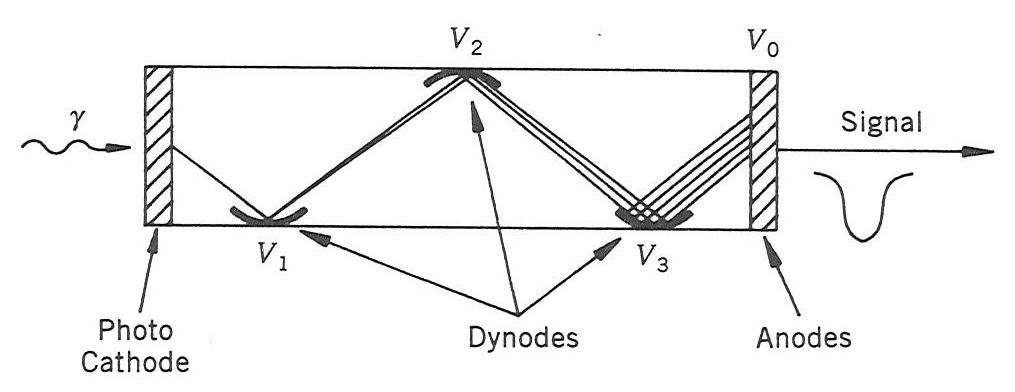
\includegraphics[scale=1.2]{figures/photomultiplier.jpg}
    \caption{Main elements of a photomultiplier tube \cite{intro_nuclear_particle_physics}.}
    \label{fig:photomultiplier}
\end{figure}

\paragraph{Gamma spectrometry}
WHAT IS THE GAMMA SPECTRUM?

When $\gamma$ rays enter the scintillator, they can interact in two possible ways: through the photoelectric effect or through Compton scattering.
Any photon converted to an electron by photoelectric effect generally deposits its entire energy within the scintillator, such that the intensity of the subsequent scintillation light is proportional to the energy of the original photon.
In the case of Compton scattering, instead, the photons do not deposit all of their energy and, once scattered, can produce new interactions.
A third way would be through $e^+ e^-$ pair production, but it is very unlikely\footnote{'Which is however very unlikely'?} for low-energy photons.

[The energy deposited in the NaI will therefore have two kinds of contributions to the $\gamma$ spectrum.
First, the full energies of any of the photons that convert into photoelectrons, and, second, a continuous spectrum of energies related to Compton scattering] \hl{$<$-- remanier un peu}



\paragraph{Experimental setup}
An inorganic scintillation detector consisting of a NaI crystal was used.
Then Amplifier, discriminateur, analyseur  multi-bande ecc\dots.

\hl{Bien expliquer les coincidences}